\documentclass{beamer}
\usetheme{Boadilla}
% \usepackage{beamerthemesplit} // Activate for custom appearance
\usepackage{mathtools}
\usepackage{amsmath}
\usepackage{amssymb}

\newcommand{\bbR}{\mathbb{R}}
\newcommand{\bbZ}{\mathbb{Z}}
\newcommand{\vb}{\vec{b}}
\newcommand{\vv}{\vec{v}}
\newcommand{\vvs}{\vec{v}^*}
\newcommand{\vbs}{\vec{b}^*}
\newcommand{\sspan}{\mathsf{span}}
\newcommand{\vol}{\mathrm{vol}}
\newcommand{\GH}{\mathrm{GH}}
\newcommand{\FEC}{\mathrm{FEC}}
\newcommand{\ENUMCost}{\mathrm{ENUMCost}}
\newcommand{\MINCost}{\mathrm{MINCost}}
\newcommand{\SimENUMCost}{\mathrm{Sim}\text{-}\mathrm{ENUMCost}}
\newcommand{\Costbeta}{\mathrm{Cost}_{\beta}}
\newcommand{\SimGSLengths}{\mathrm{Sim}\text{-}\mathrm{GS}\text{-}\mathrm{Lengths}}
\newcommand{\SimFEC}{\mathrm{Sim}\text{-}\mathrm{FEC}}
\newcommand{\SimGH}{\mathrm{Sim}\text{-}\mathrm{GH}}
\newcommand{\TimeBKZ}{\mathrm{TimeBKZ}}

\newtheorem*{remark}{Remark}

\title{Improved Progressive BKZ Algorithms and Their Precise Cost Estimation by Sharp Simulator}
\subtitle{Yoshinori Aono, Yuntao Wang, Takuya Hayashi, and Tsuyoshi Takagi}
\author{Yuncong Zhang}
\date{April 10, 2020}

\begin{document}

\frame{\titlepage}

\frame{\frametitle{Outline} \tableofcontents}

\section{Introduction}
\frame
{
  \frametitle{Introduction}
  \begin{columns}
  \begin{column}{0.6\textwidth}
  The \emph{Shortest Vector Problem} (SVP):
  \begin{itemize}
  	\item Given the lattice $L=L(\vb_1,\cdots,\vb_n)$
  	\item Find the shortest non-zero vector $\vvs\in L$, denote $\lambda_1(L):=\|\vvs\|$
  	\item $\gamma$-SVP: find $\vv$ with $\|\vv\|\leq\gamma\cdot\lambda_1(L)$
  \end{itemize}
  \end{column}
  \begin{column}{0.4\textwidth}
  \begin{figure}[tb]
  	\centering
  	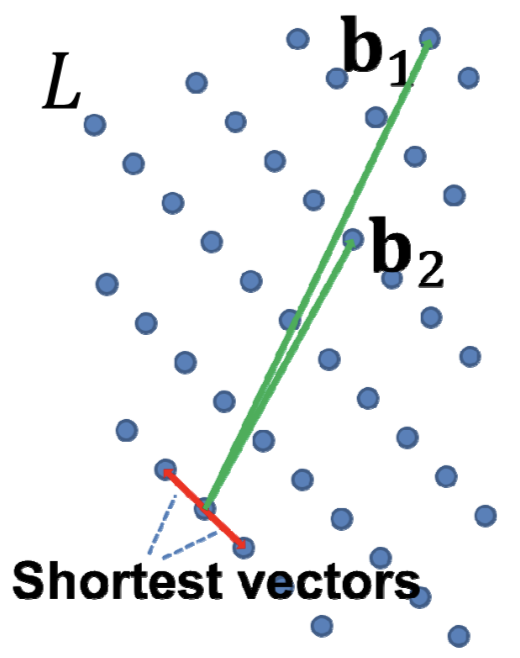
\includegraphics[width=0.8\textwidth]{files/BKZ-SVP.png}
  	\label{fig:svp}
  \end{figure}
  \end{column}
  \end{columns}
}

\frame
{
  \frametitle{Introduction}
  \begin{columns}
  \begin{column}{0.5\textwidth}

  Current algorithms for solving SVP:
  \begin{itemize}
  	\item \textbf{Blockwise (LLL, BKZ)}: Optimize the entire basis
  	\item \textbf{Enumeration}: Enumerate vectors using given basis
  	\item \textbf{Seiving}: Consumes large amount of memory, was impractical, but quite competitive now
  \end{itemize}

  \end{column}
  \begin{column}{0.5\textwidth}

  \begin{figure}[tb]
  	\centering
  	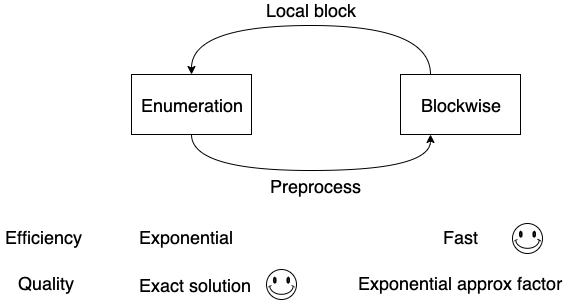
\includegraphics[width=\textwidth]{files/BKZ-SVP-Algorithms.png}
  	\label{fig:svp-alg}
  \end{figure}

  \end{column}
  \end{columns}
  \begin{block}{Remark}
  Blockwise and Enumeration algorithms rely on and compliment each other.
  \begin{itemize}
  	\item BKZ calls Enumeration on local blocks
  	\item Enumeration efficiency relies on basis quality, often require basis preprocessed by blockwise algorithm
  \end{itemize}
  \end{block}
}

\frame
{
  \frametitle{Introduction}
  History of BKZ Algorithms:
  \begin{itemize}
  	\item Basic BKZ (Schnorr 1994)
  	\item BKZ 2.0 (Chen-Nguyen 2011): a combination of improvements
  	\item Progressive BKZ: used locally in BKZ 2.0, never formally proposed as a standalone algorithm
  \end{itemize}
}

\section{Preliminaries}
\frame{
	\frametitle{Preliminaries}
	\begin{itemize}
		\item Mathematical Definitions
		\item Enumeration Algorithm
		\item LLL Algorithm
		\item Previous BKZ Algorithms
	\end{itemize}
}

\subsection{Mathematical Definitions}
\frame{
	\frametitle{Mathematical Definitions}
	Gram-Schmidt Basis for $B=(\vb_1,\cdots,\vb_n)$:
	\begin{itemize}
		\item $B^*:=(\vb_1^*,\cdots,\vb_n^*)$
		\item $\vb_i^*:=\vb_i-\sum_{j=1}^{i-1}\mu_{ij}\cdot\vb_j^*$ where $\mu_{ij}:=\langle\vb_i,\vb_j^*\rangle/\|\vb_j^*\|^2$ called GS coefficients
	\end{itemize}
	\begin{figure}[ht!]
	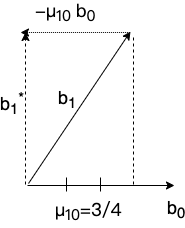
\includegraphics[width=0.2\textwidth]{files/BKZ-GS-Coeff.png}
	\caption{Example of GS coefficient $\mu_{10}$}
	\label{fig:bkz.gs.coeff}
	\end{figure}
}

\frame{
	\frametitle{Mathematical Definitions}
	Gram-Schmidt reduction preserves volume, which is volume of a lattice cell:
	\[\vol(L):=\det(L):=\det(B)=\det(B^*)=\prod_{i=1}^n \|\vb_i^*\|\]
	\begin{figure}[ht!]
	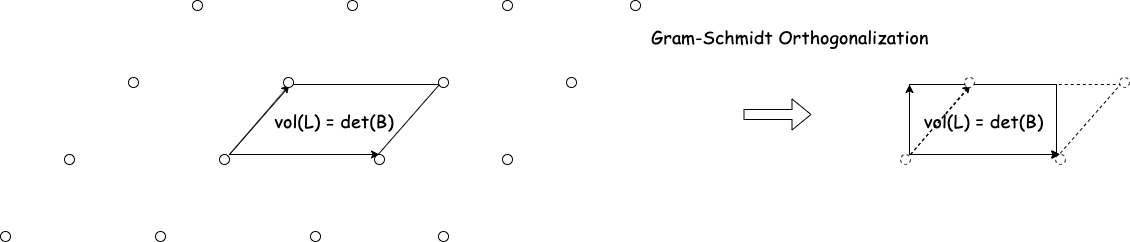
\includegraphics[width=0.8\textwidth]{files/BKZ-Volume.png}
	\caption{Gram-Schmidt orthogonalization and volume of lattice}
	\label{fig:bkz.volume}
	\end{figure}
}

\frame{
	\frametitle{Mathematical Definitions}
	Projection $\pi_i:\bbR^n\to\sspan(\vb_1,\cdots,\vb_{i-1})^{\perp}$
	\begin{eqnarray}
	\pi_i(v):=\vec{v}-\sum_{j=1}^{i-1}\langle\vec{v},\vb_j^*\rangle\vb_j^*/\|\vb_j^*\| \label{eqn:pi}
	\end{eqnarray}
	which effectively removes the proportion of the vector inside the space $\sspan(\vb_1,\cdots,\vb_{i-1})$.
	\begin{remark}
	\begin{itemize}
		\item Gram-Schmidt reduction: $\vb_i^* = \pi_i(\vb_i)$
		\item $\ker\pi_i=\sspan(\vb_1,\cdots,\vb_{i-1})$. In particular, $\pi_i(\vb_j)=0$ for $j<i$
		\item $\pi_1(\cdot)$ is the identity map
	\end{itemize}
	\end{remark}
}

\frame{
	\frametitle{Mathematical Definitions}

	\begin{figure}[ht!]
	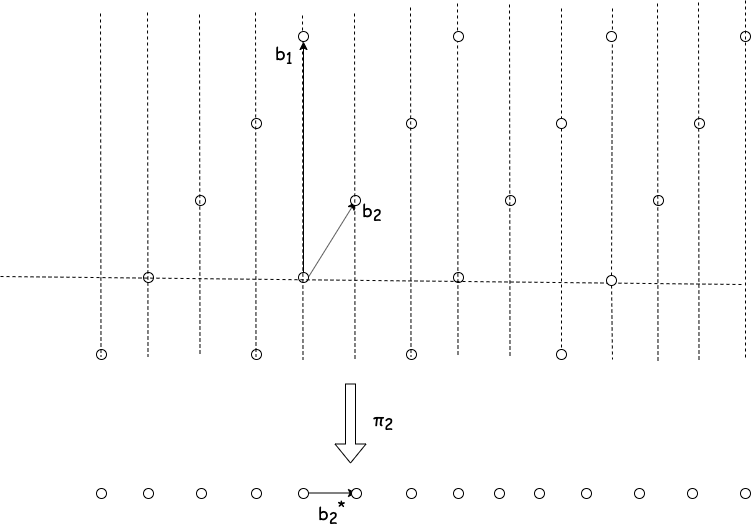
\includegraphics[width=0.7\textwidth]{files/BKZ-Projection.png}
	\caption{Projection $\pi_i$ eliminates the portion of $\vv$ in $\sspan(\vb_1,\cdots,\vb_{i-1})$}
	\label{fig:proj}
	\end{figure}
}

\frame{
	\frametitle{Mathematical Definitions}
	Projective \emph{local block} (sublattice)
	\begin{eqnarray}
	L_{[i:j]} &:=& \pi_i(L(\vb_i,\vb_{i+1},\cdots,\vb_j))
	\end{eqnarray}
	Use $B_i:=L_{[i:i+\beta-1]}$ when the blocksize $\beta$ is clear
}

\frame{
	\frametitle{Mathematical Definitions}
	Gaussian Huristic
	\begin{itemize}
		\item For convex set $S$: $|S\cap L|\approx\vol(S)/\vol(L)$
		\item Let $S$ be $n$-dimensional ball, solving $V_n(R)=\vol(L)$ gives $R=(\vol(L)/V_n(1))^{1/n}$
		\item Denote by $\GH(L):=(\vol(L)/V_n(1))^{1/n}$, approximates $\lambda_1(L)$
	\end{itemize}

	\begin{remark}
	$V_n(R)$ is the volume of the $n$-dimensional ball.
	\[V_n(R) = R^n\cdot\frac{\pi^{n/2}}{\Gamma(n/2+1)}\]
	\end{remark}
}

%\frame{
%	\frametitle{Mathematical Definitions}
%	Modified Gaussian heuristic for local blocks:
%	\begin{itemize}
%		\item For local blocks $B_i$ and small blocksize $\beta$, $\GH(B_i)$ is often smaller %than $\lambda_1(L)$
%		\item Approximates $\lambda_1(L)$ with $\tau_{\beta}\GH(B_{\beta})$ instead, where $\tau_%{\beta}$ is called modified Gaussian heuristic constant.
%		\item $\tau_{\beta}$ decreases with $\beta$ and $\tau_{\beta}\approx 1$ for $\beta>50$
%	\end{itemize}
%	% \[
%	% \tau_i:=\frac{\|\vb_{n-i+1}^*\|}{V_i(1)^{-1/i}\cdot\prod_{j=n-i+1}^n\|\vb_j^*\|^{1/i}}
%	% \]
%
%}

\subsection{Enumeration and LLL Algorithm}
\frame{
	\frametitle{Enumeration Algorithm}
	Given a lattice basis $B=(\vb_1,\cdots,\vb_n)$, finds the shortest vector $\vvs$
	\[
	\vvs=a_1\vb_1+a_2\vb_2+\cdots+a_n\vb_n\qquad\forall i\in[n]
	\]
	Observation:
	\begin{itemize}
		\item $\|\pi_n(\vvs)\|\leq\|\pi_{n-1}(\vvs)\|\leq\cdots\leq\|\pi_1(\vvs)\|=\|\vvs\|\leq R$
		\item $\pi_i(\vvs)=\pi_i(a_i\vb_i+\cdots+a_n\vb_n)$
	\end{itemize}
	% Search backwards from $a_n$
	% \begin{itemize}
	% 	\item $\pi_n(\vvs)=a_n\pi_i(\vb_n)\xRightarrow{}|a_n|\leq R/\|\vb_n^*\|$
	% 	\item For given $(a_n,\cdots,a_{i+1})\xRightarrow{}|a_i|$ is bounded
	% \end{itemize}
}

\frame{
	\frametitle{Enumeration Algorithm}
	Select radius $R$, get searching tree:
	\begin{itemize}
		\item Layer at depth $k+1$ consists of all possible $(a_n,\cdots,a_{n-k})$ s.t. $\|\pi_{n-k}(a_n\vb_n+\cdots+a_{n-k}\vb_{n-k})\|\leq R$
		\item Father-child relations: $(a_n,\cdots,a_{k+1})\to\{(a_n,\cdots,a_{k+1},a_k)\}$ for all possible $a_k$
	\end{itemize}
	\begin{figure}[ht!]
		\centering
		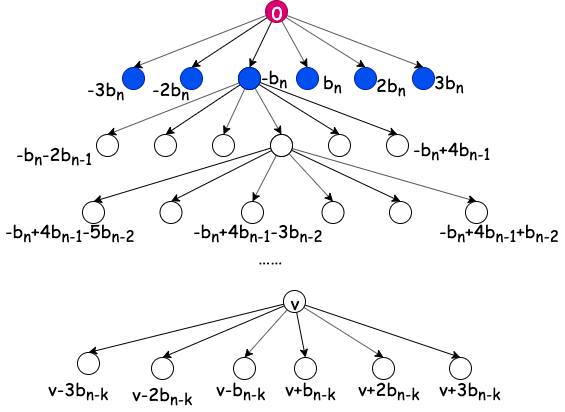
\includegraphics[width=0.4\textwidth]{files/BKZ-Searching-Tree.png}
		\caption{Searching Tree}
		\label{fig:search-tree}
	\end{figure}
}

\frame{
	\frametitle{Enumeration Algorithm}
	Cost of enumeration algorithm is measured by total number of nodes in tree, calculated by adding the size of all layers. Full Enumeration Cost (FEC) is the number of nodes when $R=\GH(L)$:

	\begin{eqnarray}
	N=\FEC(B):=\frac{1}{2}\sum_{k=1}^n \frac{V_k(\GH(L))}{\prod_{i=n-k+1}^n\|\vb_i^*\|}
	\end{eqnarray}

	\begin{itemize}
		\item $\vol(\pi_{n-k+1}(L))=\prod_{i=n-k+1}^n \|\vb_i\|$
		\item If $\vv$ is in the tree, $-\vv$ too, therefore it suffices to search only half of the tree
	\end{itemize}
}

\frame{
	\frametitle{Enumeration Algorithm}
	Pruning: select seperate bound $(R_1,\cdots,R_n)$ for each layer
	\begin{itemize}
		\item $R_n\leq R_{n-1}\leq\cdots\leq R_1=R$
		\item The pruned searching tree may fail to find any $\|\vv\|\leq R$, and has a success probability $p$ which can be estimated given $(R_1,\cdots,R_n)$
		\item For target probability $p$, radius $\alpha\cdot\GH(L)$, denote by
	\end{itemize}
	\[\ENUMCost(B;\alpha,p):=\min_{R_1,\cdots,R_n} N\]
	the minimized enumeration cost over all possible bounding functions. The minimization method is proposed by Chen-Nguyen.

	\begin{figure}[ht!]
		\centering
		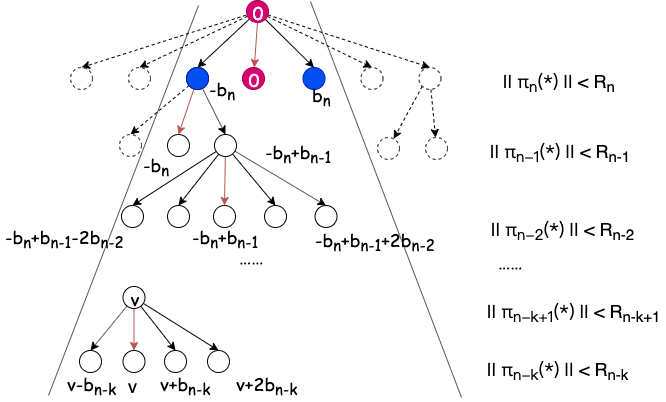
\includegraphics[width=0.4\textwidth]{files/BKZ-Pruning.png}
		\caption{Pruning Searching Tree}
		\label{fig:prune-search-tree}
	\end{figure}
}

\frame{
	\frametitle{LLL Algorithm}
	\begin{columns}
	\begin{column}{0.6\textwidth}
	On input basis $B=\{\vb_1,\cdots,\vb_n\}$, output $B'$:
	\begin{itemize}
		\item $\vb_1'$ is short
		\item $\vb_1',\cdots,\vb_n'$ are nearly orthogonal
	\end{itemize}
	\end{column}
	\begin{column}{0.4\textwidth}
	\begin{figure}[ht!]
	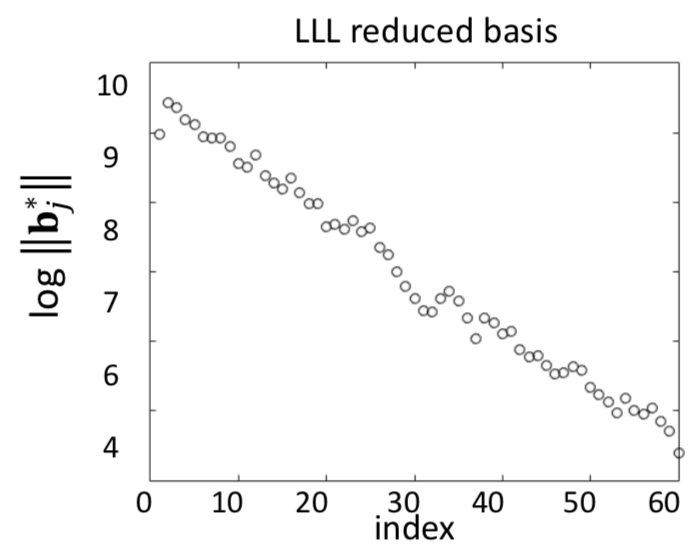
\includegraphics[width=\textwidth]{files/BKZ-LLL-Reduced.png}
	\label{fig:bkz.lll.reduced}
	\end{figure}
	\end{column}
	\end{columns}
	\begin{remark}
	Lengths of Gram-Schmidt reduced vectors are used to measure the quality of basis:
	\begin{itemize}
		\item The product $\prod_{i=1}^n\|\vb_i^*\|$ is fixed to $\vol(L)$, therefore, the size of under the curve is fixed
		\item The flatter the graph, the better the quality
	\end{itemize}
	\end{remark}
}

%\frame{
%	\frametitle{LLL Algorithm}
%	LLL (Lenstra, Lenstra, Lovasz) is a generalization of Lagrange/Gauss algorithm:
%	\begin{enumerate}
%		\item $\vb_1=\vb_1-\lfloor\mu_{1,0}\rceil\vb_0$
%		\item Swap $\vb_0$ and $\vb_1$
%		\item If $\|\vb_0\|\leq\|\vb_1\|$ and $|\mu_{1,0}|\leq 1/2$ exit; else goto 1
%	\end{enumerate}
%	\begin{figure}[ht!]
%	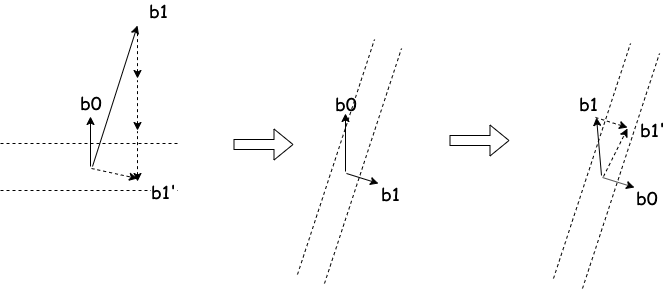
\includegraphics[width=0.6\textwidth]{files/BKZ-Lagrange.png}
%	\caption{Lagrange / Gauss Reduction}
%	\label{fig:bkz.lagrange}
%	\end{figure}
%}

%\frame{
%	\frametitle{LLL Algorithm}
%	LLL generalizes Lagrange/Gauss algorithm to $n$-dimensions.
%	\begin{itemize}
%		\item \textbf{Lovasz condition:} $\|\vb_i\|/\|\vb_{i-1}\|\geq\delta-\mu_{i,i-1}^2$, $\%delta\in(1/4,1)$
%		\item \textbf{LLL-reduced basis:} Lovasz condition, and $\mu_{i,j}\leq 1/2\quad\forall i>%j$
%	\end{itemize}
%
%	\begin{table}[ht!]
%	\begin{tabular}{p{5.5cm}p{5cm}}
%	\hline
%	\textbf{In Lagrange/Gauss algorithm} & \textbf{In LLL algorithm} \\ \hline
%	Subtract $\lfloor\mu_{1,0}\rceil\vb_0$ from $\vb_1$ & Subtracting $\lfloor\mu_{i,j}\rceil\%vb_j$ from $\vb_i$ for each $j$ from $i-1$ down to $0$ \\
%	Swap $\vb_0$ and $\vb_1$ if condition $\mu_{1,0}\leq1/2$ does not hold & Swap $\vb_{i-1}$ %and $\vb_i$ if Lovasz condition does not hold, and decrement $i$ \\
%	Succeed when condition does hold & Increment $i$ if Lovasz condition does hold for $i$ \\ \%hline
%	\end{tabular}
%	\caption{Generalization of LLL w.r.t. Lagrange/Gauss Algorithm}
%	\label{tab:gen-lll}
%	\end{table}
%}

\subsection{Previous BKZ Algorithms}
\frame{
	\frametitle{Previous BKZ Algorithms}
	\begin{itemize}
		\item Basic BKZ Algorithm
		\item BKZ 2.0
		\item Progressive BKZ
	\end{itemize}
}

\frame{
	\frametitle{Basic BKZ Algorithm}
	\begin{columns}
	\begin{column}{0.5\textwidth}
	First apply LLL on the basis.
	\end{column}
	\begin{column}{0.5\textwidth}
	\begin{figure}[ht!]
	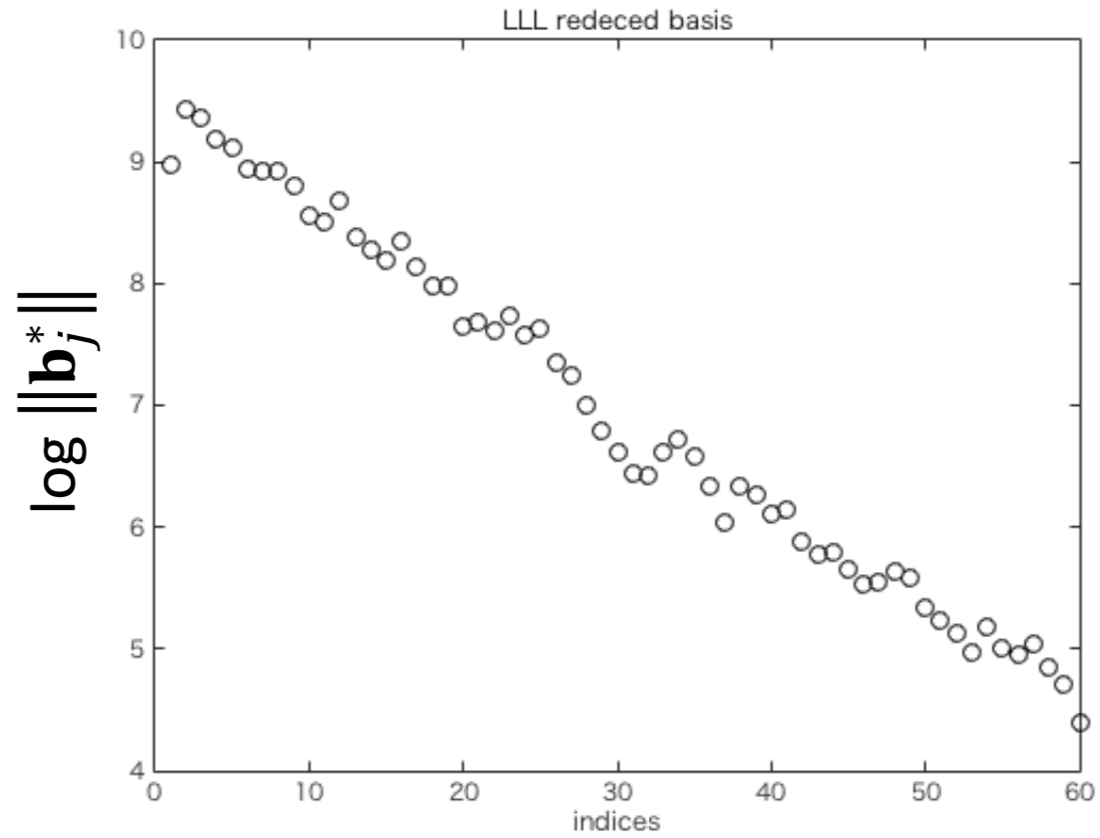
\includegraphics[width=\textwidth]{files/BKZ-Basic-1.png}
	\label{fig:bkz.basic.1}
	\end{figure}
	\end{column}
	\end{columns}
}

\frame{
	\frametitle{Basic BKZ Algorithm}
	\begin{columns}
	\begin{column}{0.5\textwidth}
	\begin{itemize}
		\item $B_1=\pi_1(L(\vb_1,\cdots,\vb_{\beta}))$
		\item $\vv\leftarrow \mathsf{ENUM}(B_1)$
		\item If $\|\vv\|\leq\|\vb_1\|$, $\alert{\mathsf{LLL}(\vv,\vb_1,\cdots,\vb_{\beta})}$
	\end{itemize}
	\end{column}
	\begin{column}{0.5\textwidth}
	\begin{figure}[ht!]
	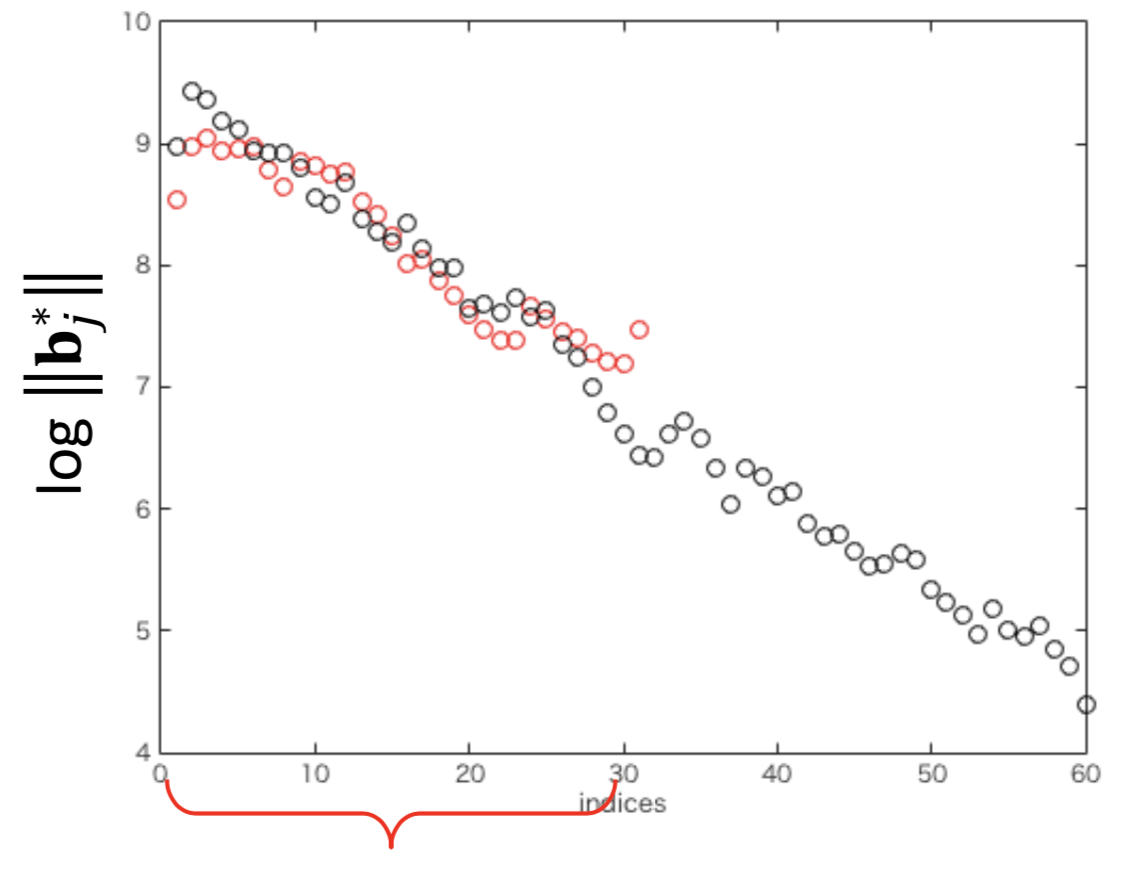
\includegraphics[width=\textwidth]{files/BKZ-Basic-2.png}
	\label{fig:bkz.basic.2}
	\end{figure}
	\end{column}
	\end{columns}
}

\frame{
	\frametitle{Basic BKZ Algorithm}
	\begin{columns}
	\begin{column}{0.5\textwidth}
	\begin{itemize}
		\item $B_2=\pi_2(L(\vb_2,\cdots,\vb_{\beta+1}))$
		\item $\pi_2(\vv)\leftarrow \mathsf{ENUM}(B_2)$
		\item If $\|\vv\|\leq\|\vb_2\|$, $\alert{\mathsf{LLL}(\vv,\vb_2,\cdots,\vb_{\beta+1})}$
	\end{itemize}
	\begin{remark}
	Assume ENUM found $\pi_2(\vv)=x_2\pi_2(\vb_2)+\cdots+x_{\beta+1}\pi_2(\vb_{\beta+1})$,
	then $\vv=x_2\vb_2+\cdots+x_{\beta+1}\vb_{\beta+1}$
	\end{remark}
	\end{column}
	\begin{column}{0.5\textwidth}
	\begin{figure}[ht!]
	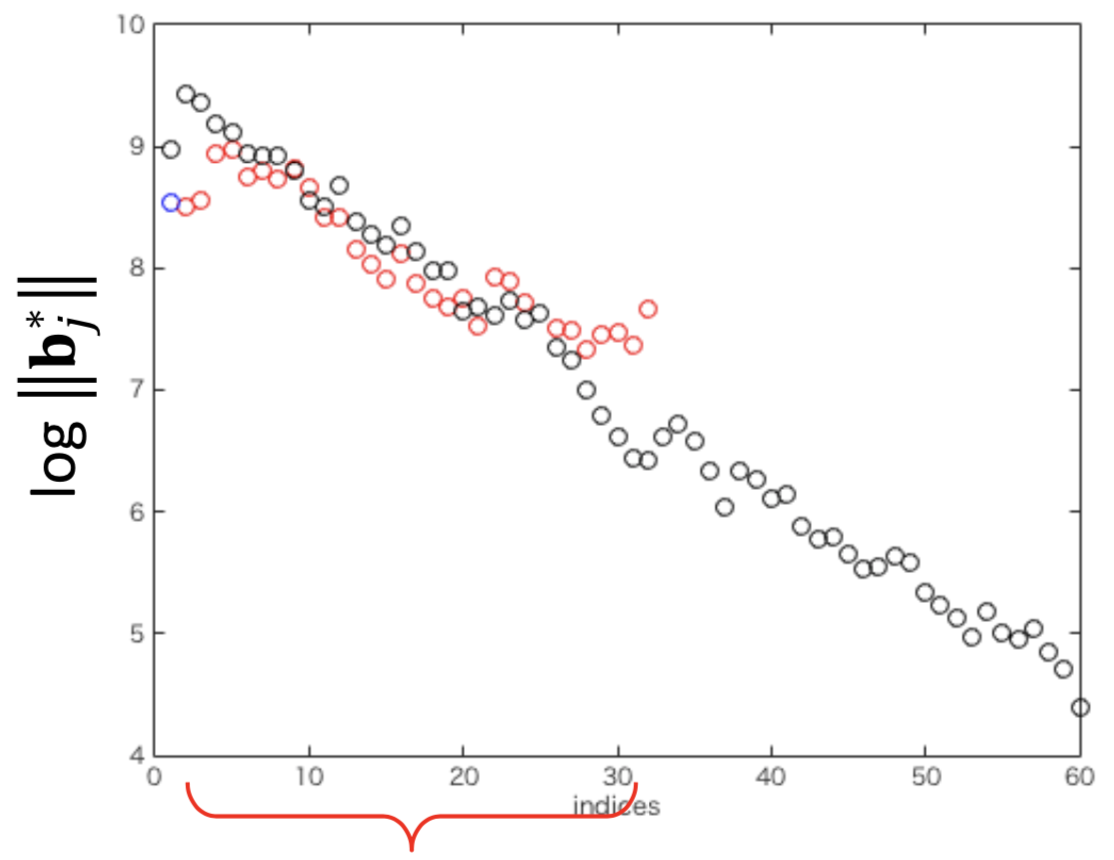
\includegraphics[width=\textwidth]{files/BKZ-Basic-3.png}
	\label{fig:bkz.basic.3}
	\end{figure}
	\end{column}
	\end{columns}
}

\frame{
	\frametitle{Basic BKZ Algorithm}
	\begin{columns}
	\begin{column}{0.5\textwidth}
	\begin{itemize}
		\item $B_3=\pi_3(L(\vb_3,\cdots,\vb_{\beta+2}))$
		\item $\pi_3(\vv)\leftarrow \mathsf{ENUM}(B_3)$
		\item If $\|\vv\|\leq\|\vb_3\|$, $\alert{\mathsf{LLL}(\vv,\vb_3,\cdots,\vb_{\beta+2})}$
	\end{itemize}
	\end{column}
	\begin{column}{0.5\textwidth}
	\begin{figure}[ht!]
	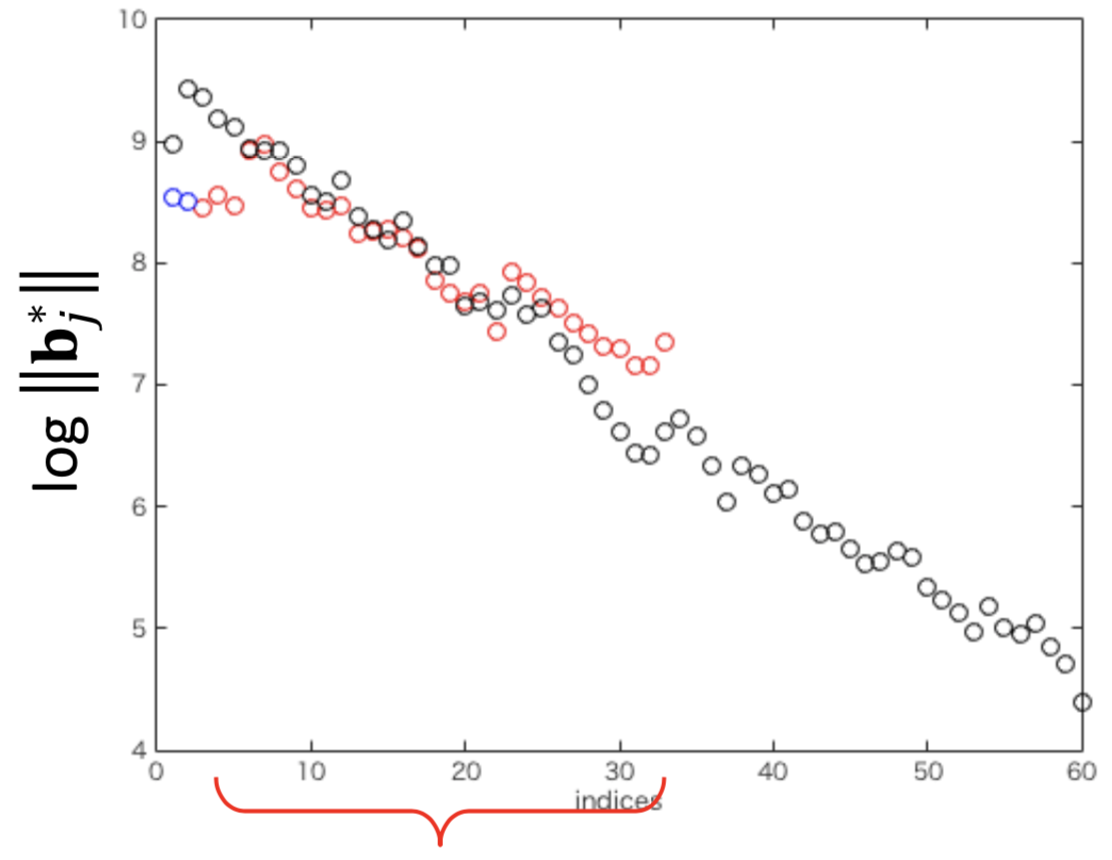
\includegraphics[width=\textwidth]{files/BKZ-Basic-4.png}
	\label{fig:bkz.basic.4}
	\end{figure}
	\end{column}
	\end{columns}
}

\frame{
	\frametitle{Basic BKZ Algorithm}
	\begin{columns}
	\begin{column}{0.5\textwidth}
	\begin{itemize}
		\item $B_{n-3}=\pi_{n-3}(L(\vb_{n-3},\cdots,\vb_n))$
		\item $\pi_{n-3}(\vv)\leftarrow \mathsf{ENUM}(B_{n-3})$
		\item If $\|\vv\|\leq\|\vb_{n-3}\|$, $\alert{\mathsf{LLL}(\vv,\vb_{n-3},\cdots,\vb_{n})}$
	\end{itemize}
	\end{column}
	\begin{column}{0.5\textwidth}
	\begin{figure}[ht!]
	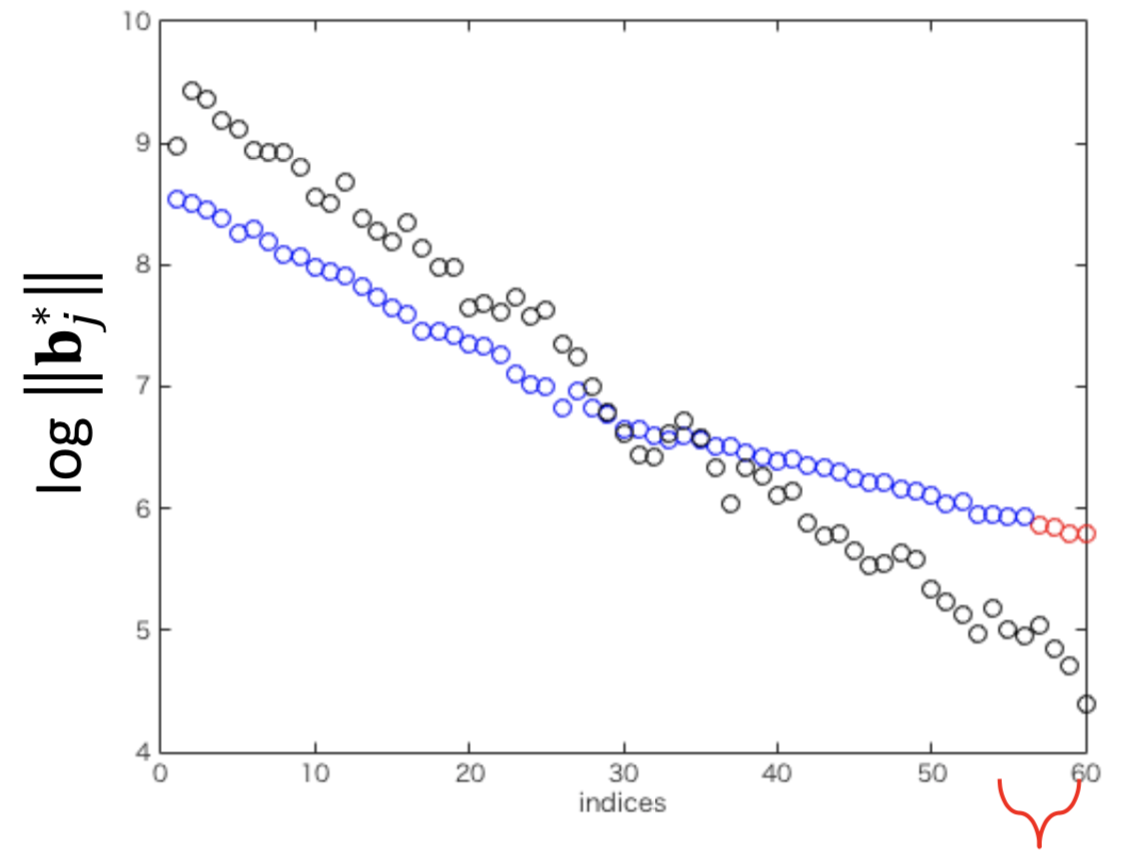
\includegraphics[width=\textwidth]{files/BKZ-Basic-5.png}
	\label{fig:bkz.basic.5}
	\end{figure}
	\end{column}
	\end{columns}
}

\frame{
	\frametitle{Basic BKZ Algorithm}
	\begin{columns}
	\begin{column}{0.5\textwidth}
	\begin{itemize}
		\item $B_{n-2}=\pi_{n-2}(L(\vb_{n-2},\vb_{n-1},\vb_n))$
		\item $\pi_{n-2}(\vv)\leftarrow \mathsf{ENUM}(B_{n-2})$
		\item If $\|\vv\|\leq\|\vb_{n-2}\|$, $\alert{\mathsf{LLL}(\vv,\vb_{n-2},\vb_{n-1},\vb_{n})}$
	\end{itemize}
	\end{column}
	\begin{column}{0.5\textwidth}
	\begin{figure}[ht!]
	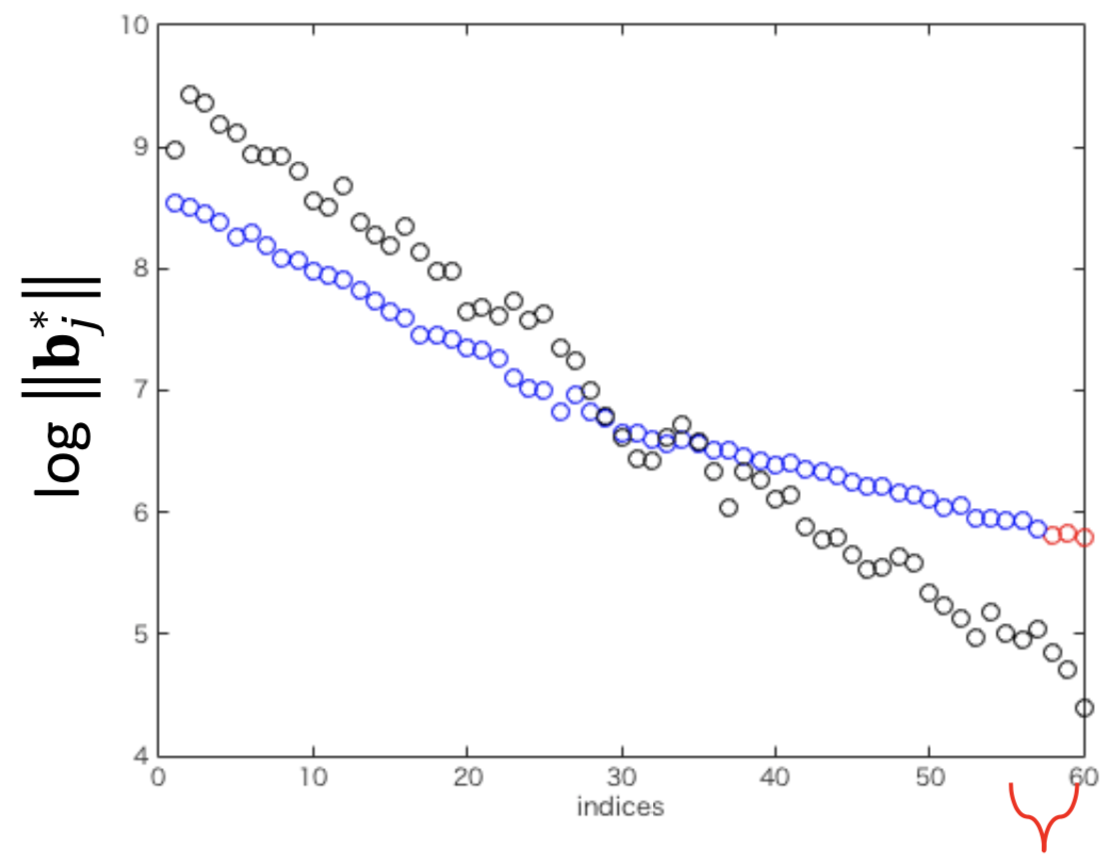
\includegraphics[width=\textwidth]{files/BKZ-Basic-6.png}
	\label{fig:bkz.basic.6}
	\end{figure}
	\end{column}
	\end{columns}
}

\frame{
	\frametitle{Basic BKZ Algorithm}
	\begin{columns}
	\begin{column}{0.5\textwidth}
	\begin{itemize}
		\item $B_{n-1}=\pi_{n-1}(L(\vb_{n-1},\vb_n))$
		\item $\pi_{n-1}(\vv)\leftarrow \mathsf{ENUM}(B_{n-1})$
		\item If $\|\vv\|\leq\|\vb_{n-1}\|$, $\alert{\mathsf{LLL}(\vv,\vb_{n-1},\cdots,\vb_{n})}$
	\end{itemize}
	\end{column}
	\begin{column}{0.5\textwidth}
	\begin{figure}[ht!]
	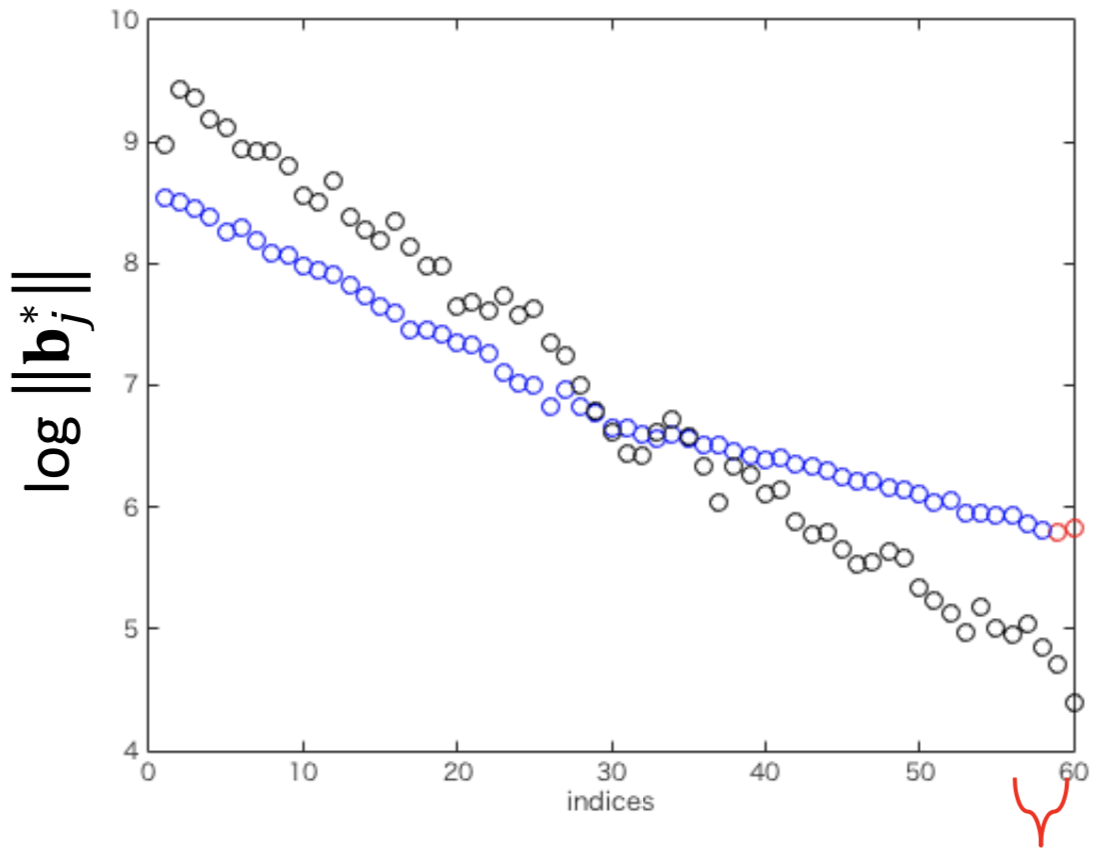
\includegraphics[width=\textwidth]{files/BKZ-Basic-7.png}
	\label{fig:bkz.basic.7}
	\end{figure}
	\end{column}
	\end{columns}
}

\frame{
	\frametitle{Basic BKZ Algorithm}
	\begin{columns}
	\begin{column}{0.5\textwidth}
	Now we complete one ROUND of BKZ.
	\end{column}
	\begin{column}{0.5\textwidth}
	\begin{figure}[ht!]
	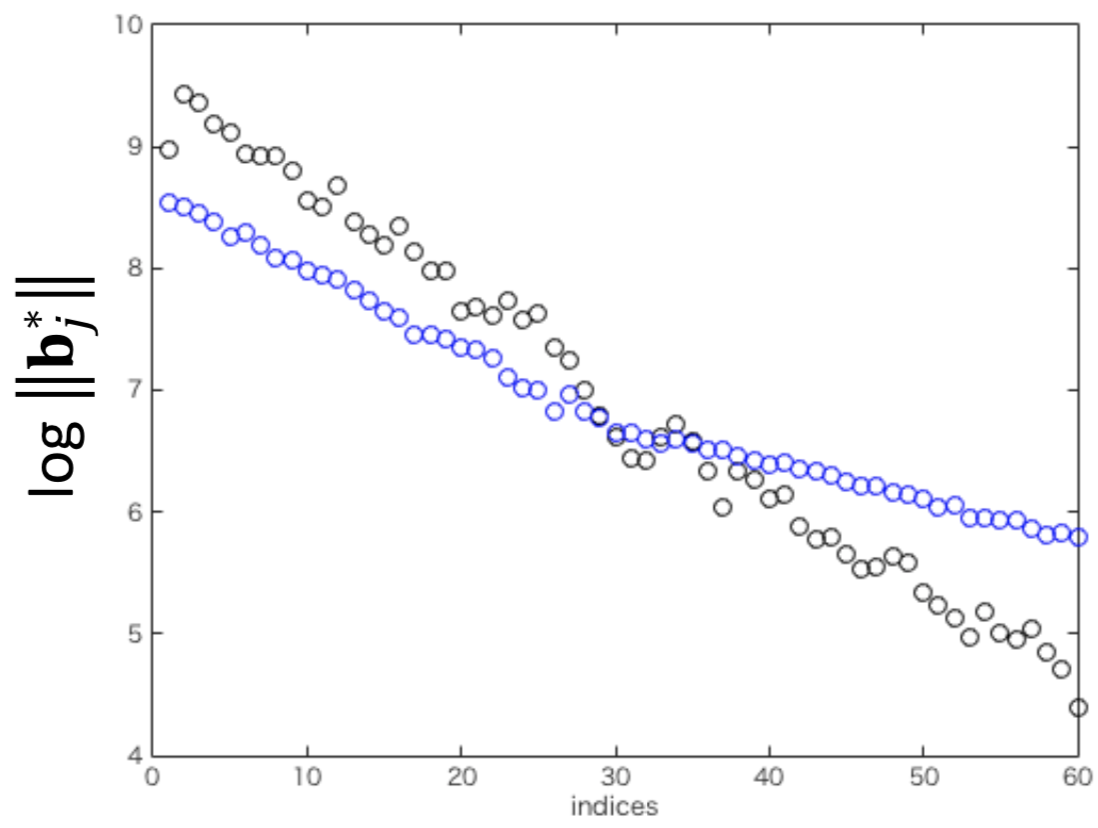
\includegraphics[width=\textwidth]{files/BKZ-Basic-8.png}
	\label{fig:bkz.basic.8}
	\end{figure}
	\end{column}
	\end{columns}
}

\frame{
	\frametitle{Basic BKZ Algorithm}
	\begin{columns}
	\begin{column}{0.5\textwidth}
	Repeat until the basis is not updated in some round. Now the basis is called \emph{BKZ-reduced}.
	\begin{block}{Definition: BKZ-reduced}
	$B=(\vb_1,\cdots,\vb_n)$ is called BKZ-$\beta$-reduced, if for each $i=1,\cdots,n$, $\vb_i^*$ is the smallest vector in $B_i$.
	\end{block}
	\end{column}
	\begin{column}{0.5\textwidth}
	\begin{figure}[ht!]
	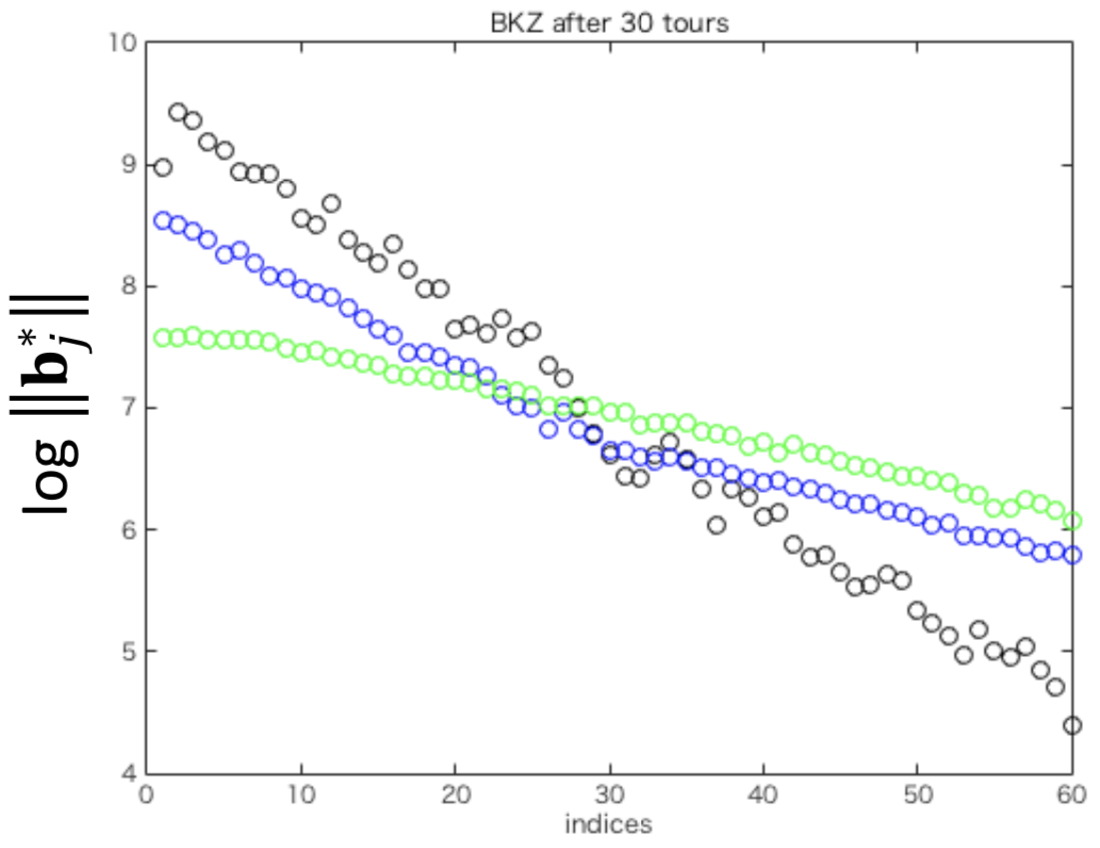
\includegraphics[width=\textwidth]{files/BKZ-Basic-9.png}
	\label{fig:bkz.basic.9}
	\end{figure}
	\end{column}
	\end{columns}
}

\frame{
	\frametitle{Basic BKZ Algorithm}
	Gram-Schmidt Assumption (GSA): for BKZ-reduced basis $B$, $\|\vb_i^*\|^2/\|\vb_1\|^2=r^{i-1}$, where $r\in[3/4,1)$ is GSA constant.
	\begin{figure}[ht!]
	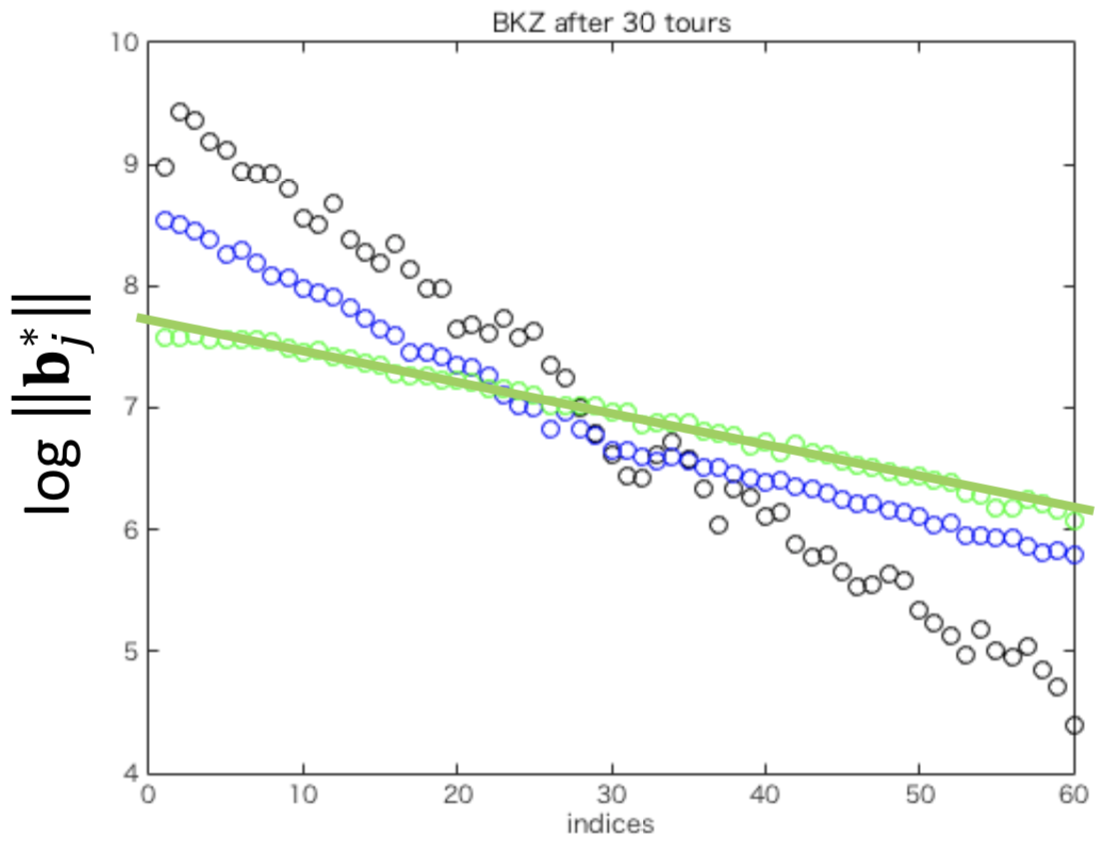
\includegraphics[width=0.6\textwidth]{files/BKZ-GSA.png}
	\label{fig:bkz.gsa}
	\end{figure}
}

\frame{
	\frametitle{BKZ 2.0}
	Proposed by Chen-Nguyen in AC 2011.
	\begin{itemize}
		\item Improvements
			\begin{itemize}
				\item \textbf{Extreme pruning} in enumeration: randomize $B_i$ to $M$ different blocks, and apply enumeration to each with extremely low probability $p=1/M$
				\item \textbf{Set searching radius} $R=\alpha\cdot\GH(B_i)\quad\alpha=\sqrt{1.1}$ based on observation that usually $\lambda_1(B_i)\leq 1.05\GH(B_i)$
				\item \textbf{Early termination}, based on observation that the basis quality is already close to the final result long before the algorithm ends
				\item \textbf{Preprocessing local blocks} using BKZ recursively with smaller blocksizes
			\end{itemize}
		\item BKZ 2.0 Simulator
			\begin{itemize}
				\item The computational cost of BKZ is hard to express in close formula, better to be estimated by simulator
				\item Execute the BKZ algorithm, modifying simulated GS lengths $\ell_1,\cdots,\ell_n$ instead of the basis $B$
			\end{itemize}
	\end{itemize}
}

\frame{
	\frametitle{Progressive BKZ}
	Observation behind progressive technique:
	\begin{itemize}
		\item Larger blocksize $\beta$ produces $\vv$ with higher quality
		\item For fixed blocksize $\beta$, the enumeration cost decreases with rounds, because the efficiency increases with quality of basis
		\item Increasing blocksize to trade efficiency for quality of $\vv$
	\end{itemize}

	\begin{figure}[ht!]
	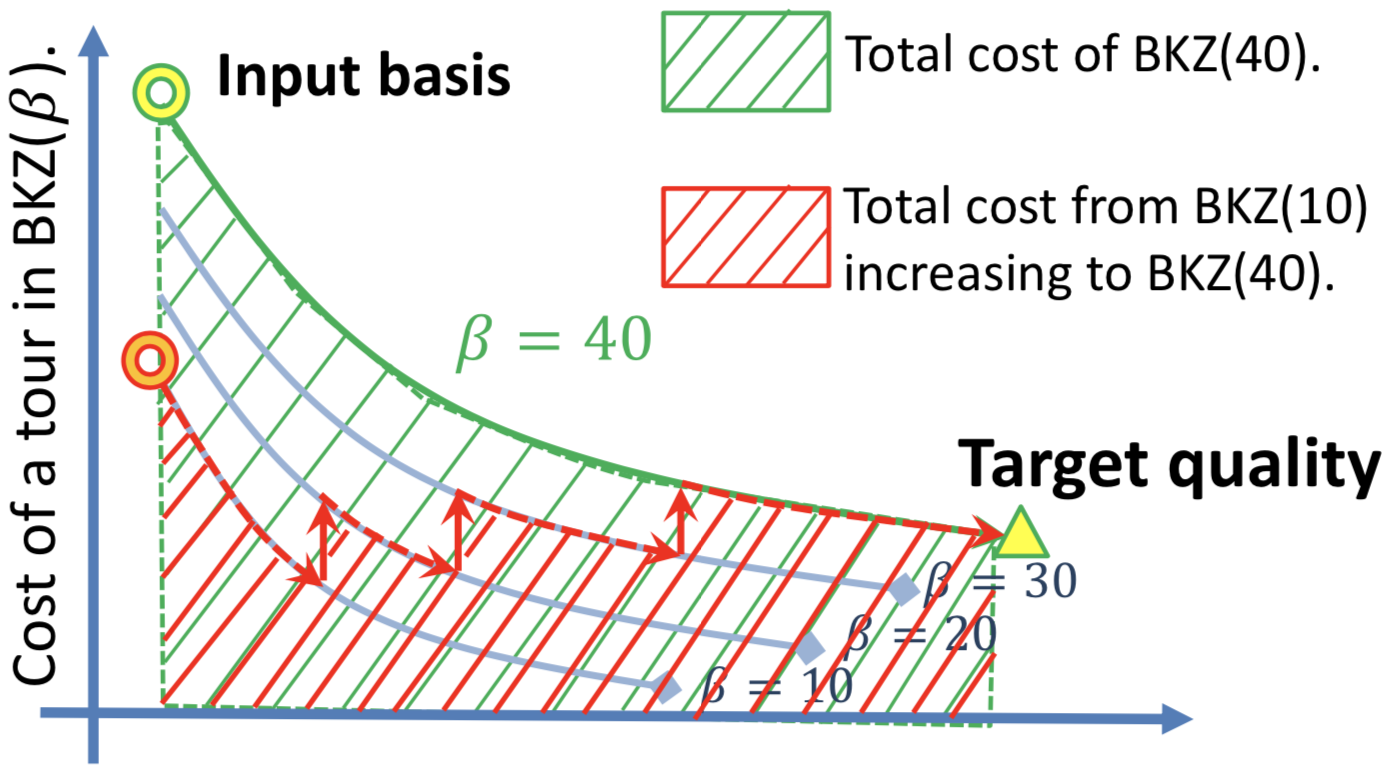
\includegraphics[width=0.6\textwidth]{files/BKZ-Progressive.png}
	\label{fig:bkz.prog}
	\end{figure}
}

\section{Improved Progressive BKZ}
\frame{
	\frametitle{Improved Progressive BKZ}
	\begin{itemize}
		\item Optimizations
		\item Implementation Detail
		\item Simulation And Comparison
	\end{itemize}
}

\subsection{Optimizations}
\frame{
	\frametitle{Optimizations}
	\begin{itemize}
		\item Optimizing Parameters
		\item Sharp Simulator
		\item Blocksize Strategy
	\end{itemize}
}

\frame{
	\frametitle{Optimizing Parameters}

	\begin{columns}
	\begin{column}{0.5\textwidth}

	Parameters inside a BKZ round:
	\begin{itemize}
		\item $\alpha$: search radius
		\item $\beta$: block size
		\item $p$: success probability
		\item $r$: GSA constant
	\end{itemize}

	\end{column}
	\begin{column}{0.5\textwidth}
	For fixed $(\beta,r)$:
	\begin{enumerate}
		\item Solve for $\alpha$ by (\ref{eqn:r-alpha-beta})
		\item Calculate $p$ by (\ref{eqn:p-alpha})
		\item Compute $\ENUMCost(B;\alpha,p)$
	\end{enumerate}

	\end{column}
	\end{columns}

	\begin{eqnarray}
	p&=&\frac{2}{\alpha^{\beta}} \label{eqn:p-alpha}\\
	r&=&\left(\frac{\beta+1}{\alpha\beta}\right)^{\frac{4}{\beta-1}}\cdot V_{\beta}(1)^{\frac{4}{\beta(\beta-1)}} \label{eqn:r-alpha-beta}
	\end{eqnarray}

}

\frame{{}
	\frametitle{Optimizing Parameters}
	Given blocksize $\beta$, find $r$ that minimizes $\ENUMCost(B;\alpha,p)$.

	\begin{figure}[ht!]
	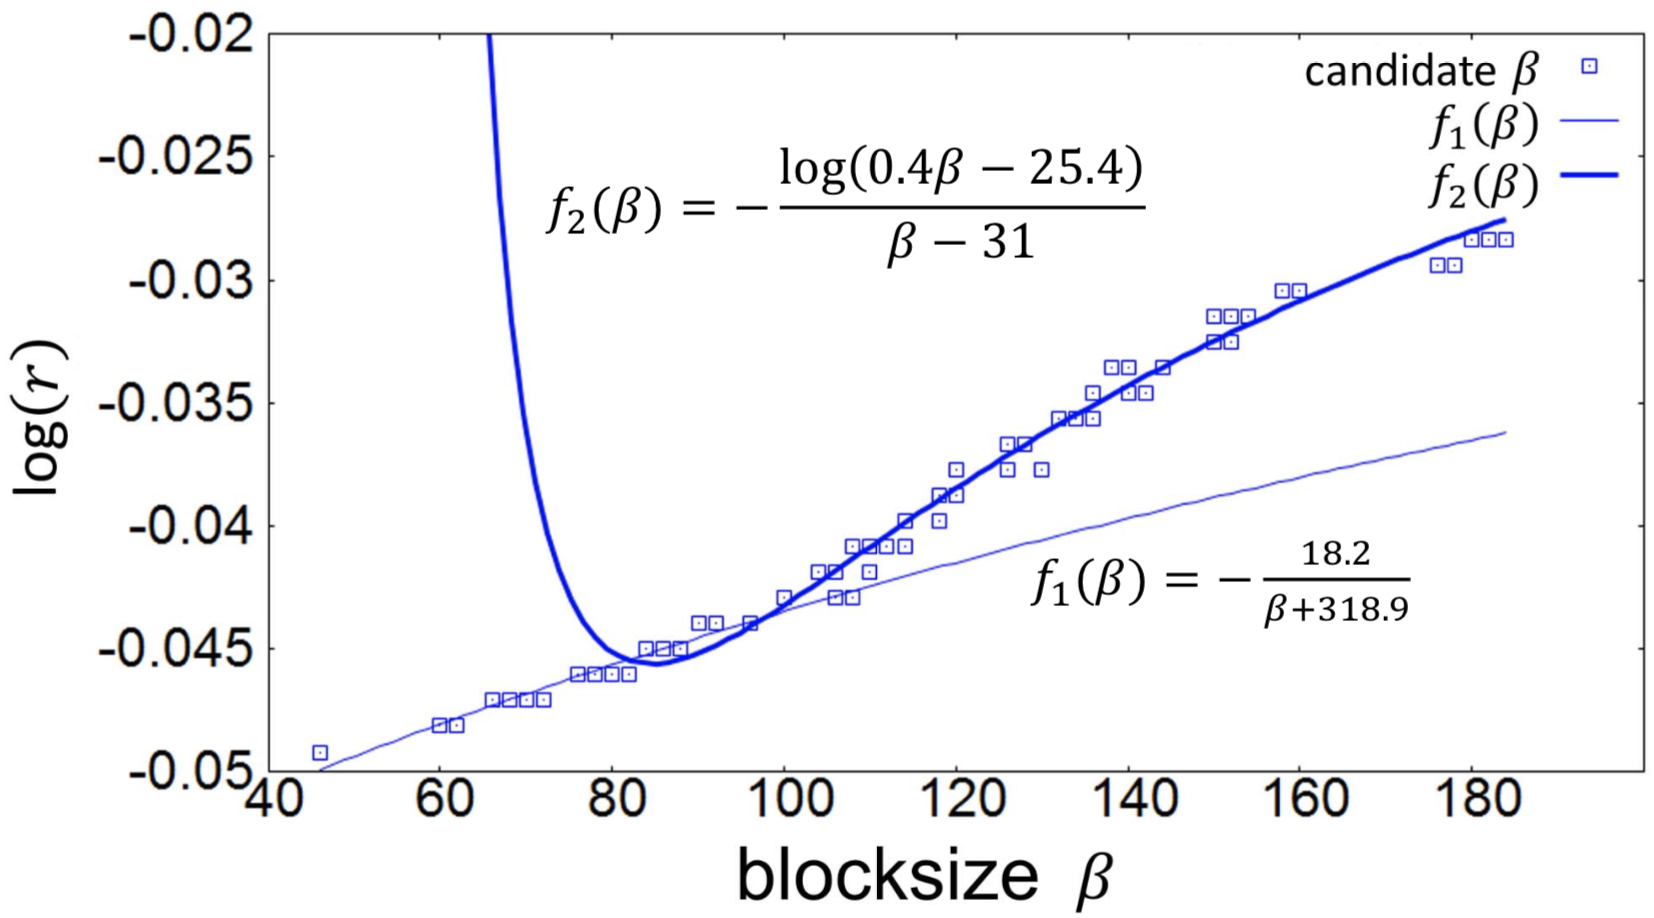
\includegraphics[width=0.6\textwidth]{files/BKZ-beta-r.png}
	\label{fig:bkz.beta.r}
	\end{figure}
	\begin{eqnarray}
	\log(r) =\left\{\begin{array}{ll}f_1(\beta)=\dfrac{-18.2139}{\beta + 318.978} & \beta\leq 100 \\\\ f_2(\beta)=\dfrac{−1.06889}{\beta - 31.0345} \cdot \log(0.417419\beta - 25.4889) & \beta > 100\end{array}\right. \label{eqn:f-beta}
	\end{eqnarray}
}

\frame{
	\frametitle{Sharp Simulator}
	Full Enumeration Cost:
	\begin{eqnarray}
	\FEC(B) := \frac{1}{2}\sum_{k=1}^n \frac{V_k(\GH(L))}{\prod_{i=n-k+1}^n \|\vb_i^*\|}
	\end{eqnarray}
	Simulated Enumeration Cost:
	\begin{eqnarray}
	\SimFEC(\ell_1,\cdots,\ell_n)&:=&\sum_{k=1}^n\frac{V_k(\SimGH(\ell_1,\cdots,\ell_n))}{\prod_{i=n-k+1}^n \ell_i}\\
	\SimGH(\ell_1,\cdots,\ell_n)&:=&\sum_{k=1}^n V_n(1)^{1/n}\prod_{j=1}^n \ell_j^{1/n}\\
	\ell_1,\cdots,\ell_n&:=&\SimGSLengths(n,\beta)
	\end{eqnarray}

}

%\frame{
%	\frametitle{Sharp Simulator}
%	Simulate Gram-Schmidt Lengths
%	\begin{itemize}
%		\item First let $\ell_n=1$, then compute $\ell_i$ backwards by solving
%		\begin{eqnarray}
%		\ell_i=\max\left\{\frac{\beta'}{\beta'+1}\alpha,\tau_{\beta'}\right\}\cdot\GH(\ell_i,\%cdots,\ell_{i+\beta'-1}) \label{eqn:sim-gs}
%		\end{eqnarray}
%		where $\beta'=\min(\beta,n-i+1)$.
%		\item Then, modify $\ell_i$ for small and big $i$
%	\end{itemize}
%}

\frame{
	\frametitle{Sharp Simulator}
	\begin{figure}[ht!]
	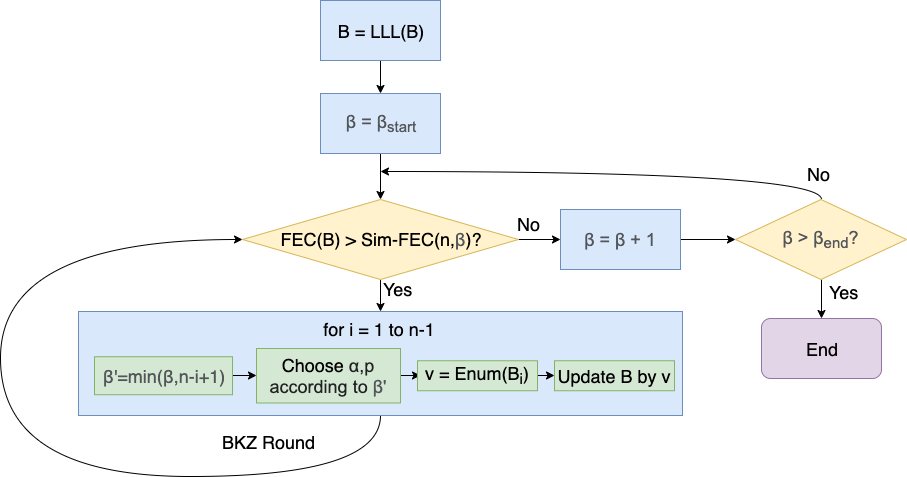
\includegraphics[width=\textwidth]{files/BKZ-Progressive-Variant.png}
	\caption{Basic Variant}
	\label{fig:bkz.prog.var}
	\end{figure}
}

\frame{
	\frametitle{Blocksize Strategy}
	A blocksize strategy is a list $\{(\beta_i^{alg},\beta_i^{goal})\}_{i=1}^D$
	\begin{itemize}
		\item Call the basis $\beta$-reduced if $\FEC(B)\leq\SimFEC(n,\beta)$
		\item At the start of strategy $i$, the basis is $\beta_{i-1}^{goal}$-reduced (except for $i=1$ where $B$ is LLL-reduced)
		\item Apply BKZ rounds to $B$ with blocksize $\beta^{alg}$, until the basis is $\beta_i^{goal}$-reduced
		\item Move to the next strategy, i.e. $i=i+1$
	\end{itemize}
	The basic variant uses the simple strategy:
	\begin{eqnarray}
	\text{LLL-reduced}\xrightarrow{\beta^{start}}\beta^{start}+1\xrightarrow{\beta^{start}+1}\cdots
	\beta^{end}-1\xrightarrow{\beta^{end}-1}\beta^{end} \nonumber
	\end{eqnarray}
}

\frame{
	\frametitle{Blocksize Strategy}
	\begin{figure}[ht!]
	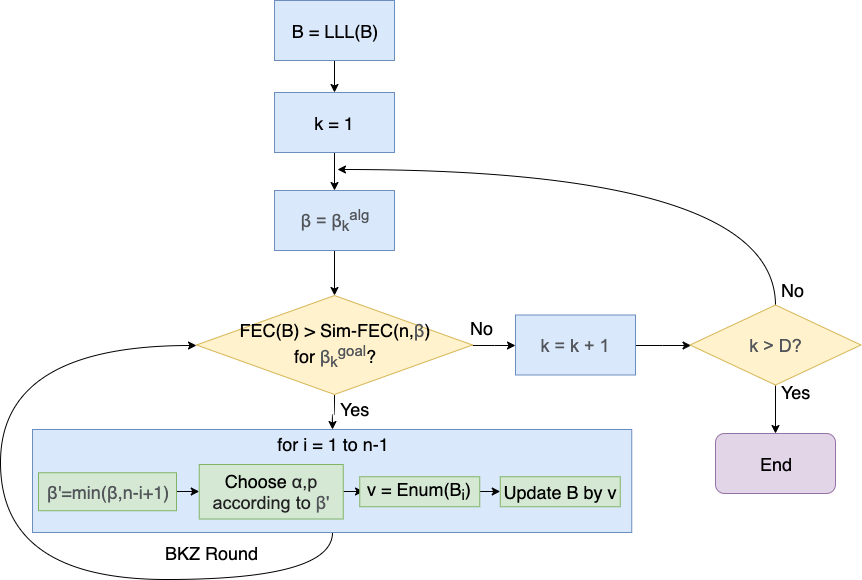
\includegraphics[width=0.8\textwidth]{files/BKZ-Blocksize-Strategy.png}
	\caption{Progressive BKZ with Blocksize Strategy}
	\label{fig:bkz.prog.strategy}
	\end{figure}
}

% \frame{
% 	\frametitle{Blocksize Strategy}
% 	$\TimeBKZ(n,\beta_{i-1}^{goal}\xrightarrow{\beta_i^{alg}}\beta_i^{goal})$: the time for % the BKZ rounds with given strategy.
%
% 	Optimizing block strategy by minimizing the total time:
% 	\begin{eqnarray}
% 	\TimeBKZ(n,\beta^{goal})=\sum_{i=1}^D\TimeBKZ(n,\beta_{i-1}^{goal}\xrightarrow{\beta_i^{alg% }}\beta_i^{goal})
% 	\end{eqnarray}
% 	By expressing the above recursively as:
% 	\begin{eqnarray}
% 	&&\TimeBKZ(n,\beta^{goal})=\nonumber\\
% 	&&\min_{\beta',\beta^{goal}}\left\{\TimeBKZ(n,\beta')+\TimeBKZ(n,\beta'\xrightarrow{\beta^{% alg}}\beta^{goal})\right\} \nonumber
% 	\end{eqnarray}
% 	We can compute $\TimeBKZ(n,\beta^{goal})$ in a dynamic programming way.
% }

% \frame{
% 	\frametitle{Blocksize Strategy}
% 	However, when blocksize is larger than $100$
% 	\begin{itemize}
% 		\item The optimized blocksize strategy is close to the simple blocksize strategy
% 		\item The overall is worse due to heavy computation in the optimization
% 	\end{itemize}
% }

\subsection{Implementation Detail}
% \frame{
% 	\frametitle{Implementation Detail}
% 	Implementation of a single BKZ iteration consists of the following steps:
% 	\begin{itemize}
% 		\item Choose parameters
% 		\item Preprocess local block
% 		\item Enumeration
% 		\item LLL reduction
% 	\end{itemize}
% }
%
% \frame{
% 	\frametitle{Implementation Detail}
% 	\begin{figure}[ht!]
% 	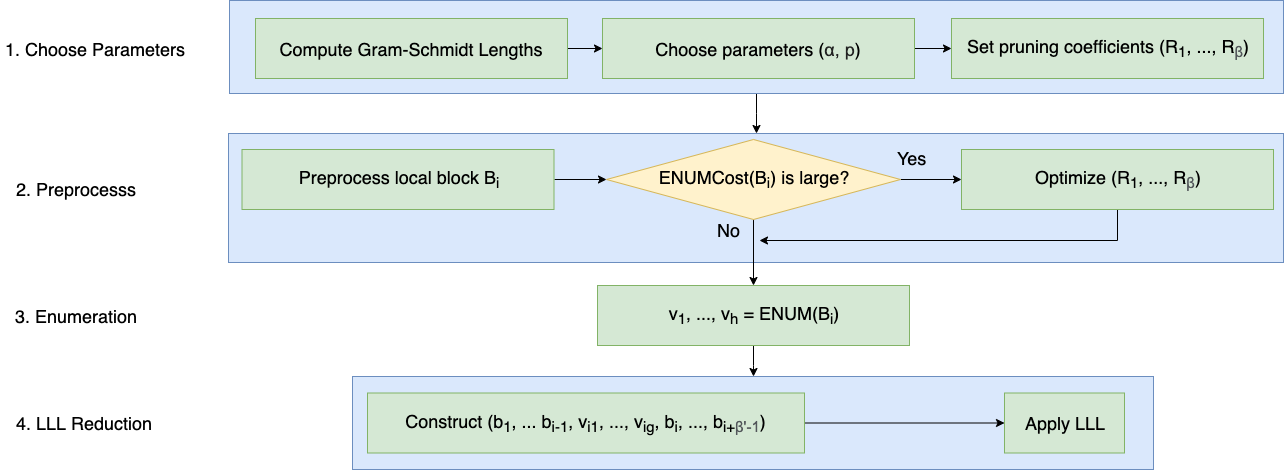
\includegraphics[width=\textwidth]{files/BKZ-Round-Detail.png}
% 	\caption{Round Implemention Detail}
% 	\label{fig:bkz.round.detail}
% 	\end{figure}
% }

% \frame{
% 	\frametitle{Implementation Detail}
% 	Choose Parameters
% 	\begin{enumerate}
% 		\item \textbf{Compute Gram-Schmidt lengths.} Compute the Gram-Schmidt variables $\|\vb_i^% *\|$ and $\mu_{ij}$ for the local block $B_i$.
% 		\item \textbf{Choose parameters $\alpha,p$.} According to equations (\ref{eqn:p-alpha})(\% ref{eqn:r-alpha-beta}) and (\ref{eqn:f-beta}).
% 		\item \textbf{Compute bounding coefficients.} Compute $(R_1,\cdots,R_{\beta})$ using % Chen-Nguyen's minimization method.
% 	\end{enumerate}
% 	The costs of these steps are negligible.
% }

\frame{
	\frametitle{Implementation Detail}
	Preprocessing
	\begin{enumerate}
		\item Preprocess the local block $B_i$ using this improved progressive BKZ algorithm, with much smaller blocksizes.
		\item The blocksize strategy takes the simple one-by-one strategy starting from $15$.
		% \item Estimate the main enumeration cost, and if the cost is too large, optimize $(R_1,\cdots,R_{\beta})$.
	\end{enumerate}
	The cost of this step: a constant $A_{Preprocess}$ times the main enumeration cost.
}

\frame{
	\frametitle{Implementation Detail}
	Enumeration
	\begin{itemize}
		\item Outputs $h=16$ vectors $(\vv_1,\cdots,\vv_h)$ with small projective lengths, instead of only one $\vv$ in original BKZ
		\item The cost is \[A_{Enum}\cdot\beta\cdot\ENUMCost(B_i;\alpha,p)\]where $A_{Enum}$ is a constant
	\end{itemize}
}

\frame{
	\frametitle{Implementation Detail}
	Construct degenerated basis by inserting some of $(\vv_1,\cdots,\vv_h)$ into the basis
	\begin{itemize}
		\item Select $g$ elements $(\vv_{i_1},\cdots,\vv_{i_g})$ from $(\vv_1,\cdots,\vv_h)$ and insert into the $i$'th position of $(\vb_1,\cdots,\vb_{i+\beta'-1})$ as follows
		\item Each $\vv_{i_j}$ is selected to minimize $\pi'(\vv_{i_j})$, and require that $\|\pi'(\vv_{i_j})\|<\|\vv_{i_{j-1}}\|$, where $\pi'$ maps $\vv$ to its projection on $\sspan(\vb_1,\cdots,\vb_{i-1}, \vv_{i_1}, \cdots, \vv_{i_{j-1}})$
		\item Stop if none of the left $\vv_i$'s satisfies the requirement
	\end{itemize}
	\begin{figure}[ht!]
	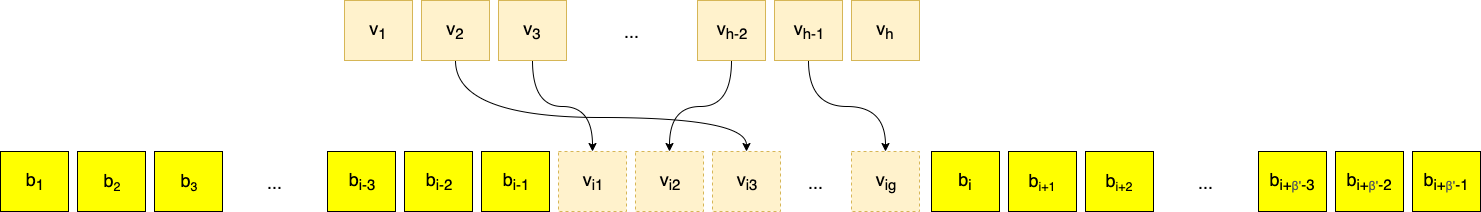
\includegraphics[width=\textwidth]{files/BKZ-Degenerate.png}
	\label{fig:bkz.degenerate}
	\end{figure}
}

\frame{
	\frametitle{Implementation Detail}
	Apply LLL:
	\begin{itemize}
		\item The first $i-1$ vectors in the degenerated basis is already LLL-reduced
		\item The cost is $A_1\cdot\beta^2 n^2$, where $A_1$ is constant
	\end{itemize}
}

\frame{
	\frametitle{Implementation Detail}
	Total cost estimation:
	\begin{eqnarray}
	&&\mathrm{Time}(n,\beta,A_1,W_1)\nonumber\\&&=\sum_{\beta^{start}}^{\beta^{goal}}\sum_{t=1}^{\#rounds}
	\left[A_1\cdot\beta^2 n^3+W_1\cdot\beta\sum_{i=1}^{n-1}\ENUMCost(B_i;\alpha,p)\right] \nonumber
	\end{eqnarray}
	where $A_1$ and $W_1$ are constants that are determined by experiments.
	\begin{itemize}
		\item The coefficients are fitted by standard curve fitting method in semi-log scale.
		\item Fitting results: $A_1=1.5\cdot 10^{-10}$ and $W_1=1.5\cdot 10^{-8}$.
	\end{itemize}
}

\frame{
	\frametitle{Pre/Post-Processing}
	A complete attack on the SVP consists of two steps:
	\begin{enumerate}
		\item Apply BKZ reduction to the basis
		\item Use enumeration to find a short vector
	\end{enumerate}
	The Preprocessing and Postprocessing works similar to extreme pruning:
	\begin{itemize}
		\item \textbf{Preprocessing}: Randomize $B_i$ to $M$ different basis
		\item \textbf{BKZ}: Apply the improved progressive BKZ to all the $B_i$'s
		\item \textbf{Postprocessing}: Apply enumeration with probability $p=2\cdot\alpha^{-n}/M$
	\end{itemize}
}

\subsection{Simulation and Comparison}
\frame{
	\frametitle{Simulation Results for SVP Challenges}
	This is the comparison result of \textbf{simulated} results, where Lindner-Peikert's estimation is the cost estimation of the basic BKZ.
	\begin{figure}[ht!]
	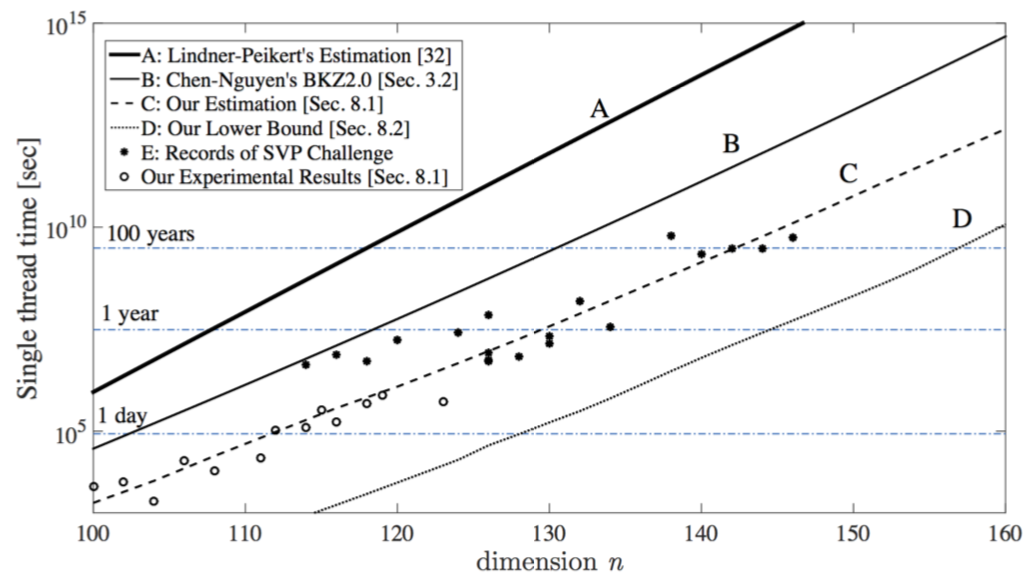
\includegraphics[width=0.6\textwidth]{files/BKZ-Comparison.png}
	\label{fig:bkz.comparison}
	\end{figure}
}


\frame{
	\frametitle{Real Results}
	\begin{figure}[ht!]
	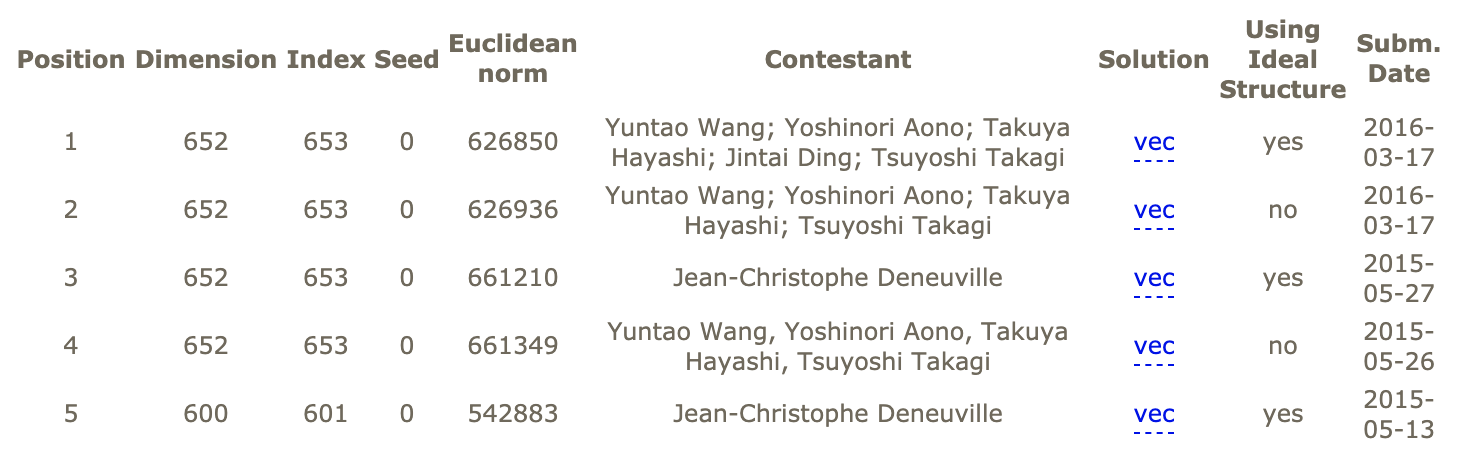
\includegraphics[width=0.6\textwidth]{files/BKZ-Ideal-Lattice-Challenge.png}
	\caption{Ideal Lattice Challenge}
	\label{fig:bkz.ideal.lattice}
	\end{figure}
	\begin{figure}[ht!]
	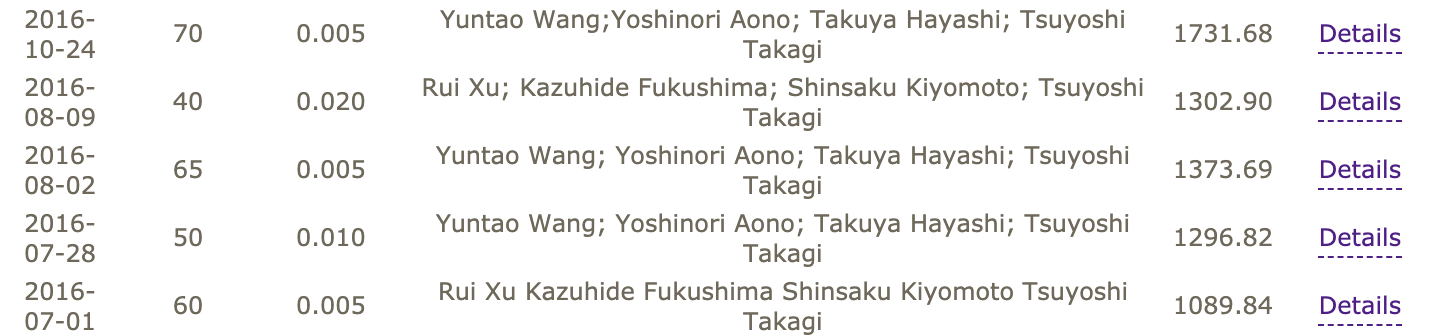
\includegraphics[width=0.6\textwidth]{files/BKZ-LWE-Challenge.png}
	\caption{LWE Challenge}
	\label{fig:bkz.lwe}
	\end{figure}
}


\frame{
	\center
	\large{Q \& A}
}

\end{document}
